\section{ICD Sensing}
\label{sec:sensing}
\begin{figure}[t]
	\centering
	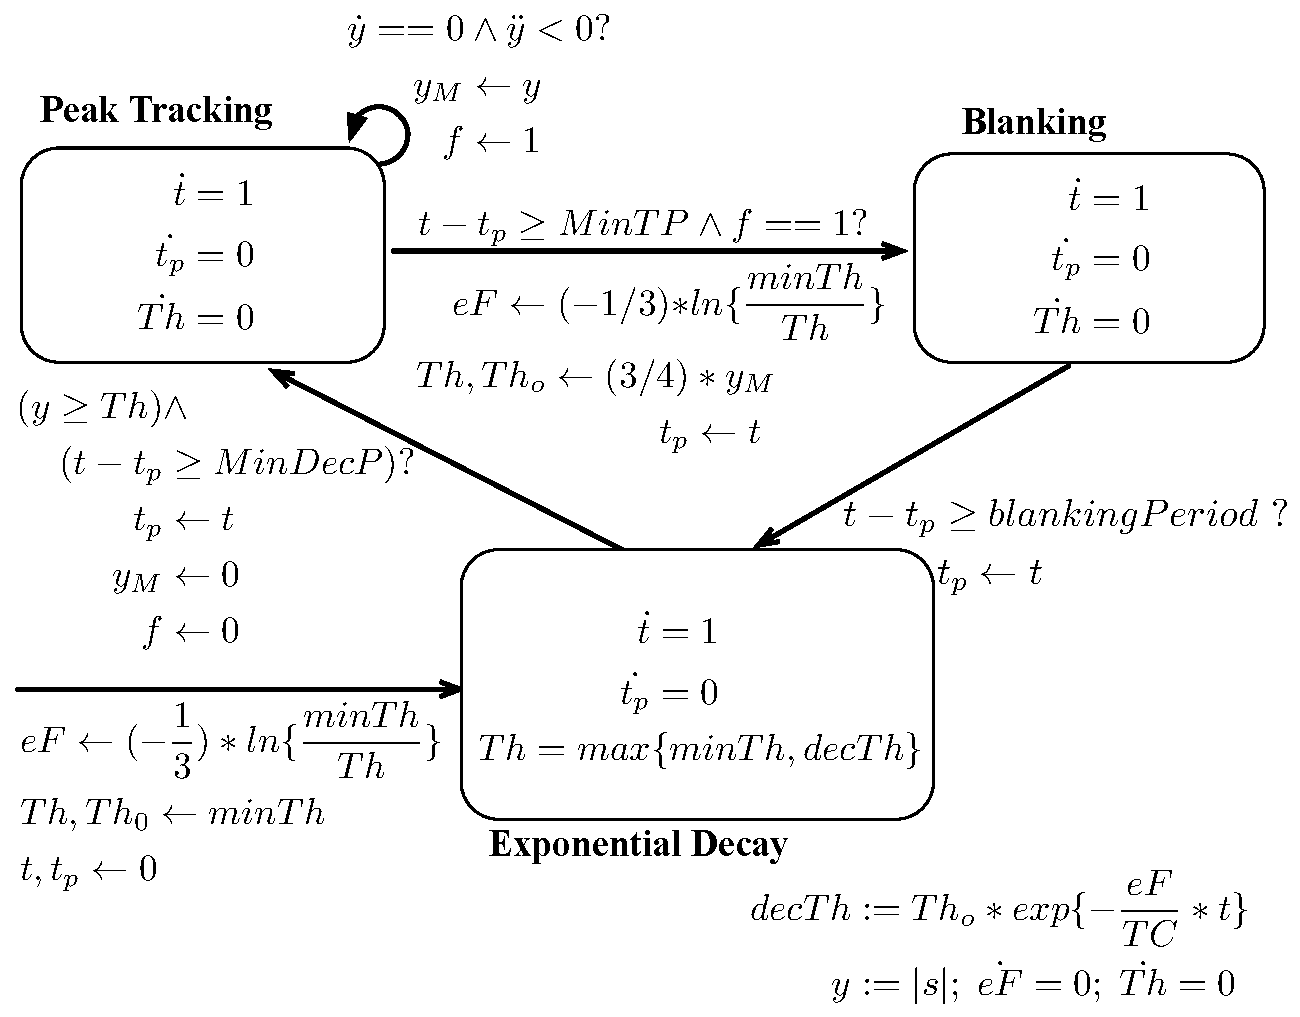
\includegraphics[scale=0.35]{figures/sensingModel}
	\vspace{-10pt}
	\caption{\small $\Sys_{Sense}$. States not shown in a mode have a 0 derivative, e.g., $\dot{eF}=0$ in all modes.}
	\vspace{-10pt}
	\label{fig:sensingModel}
\end{figure}
\begin{figure}[t]
	\centering
	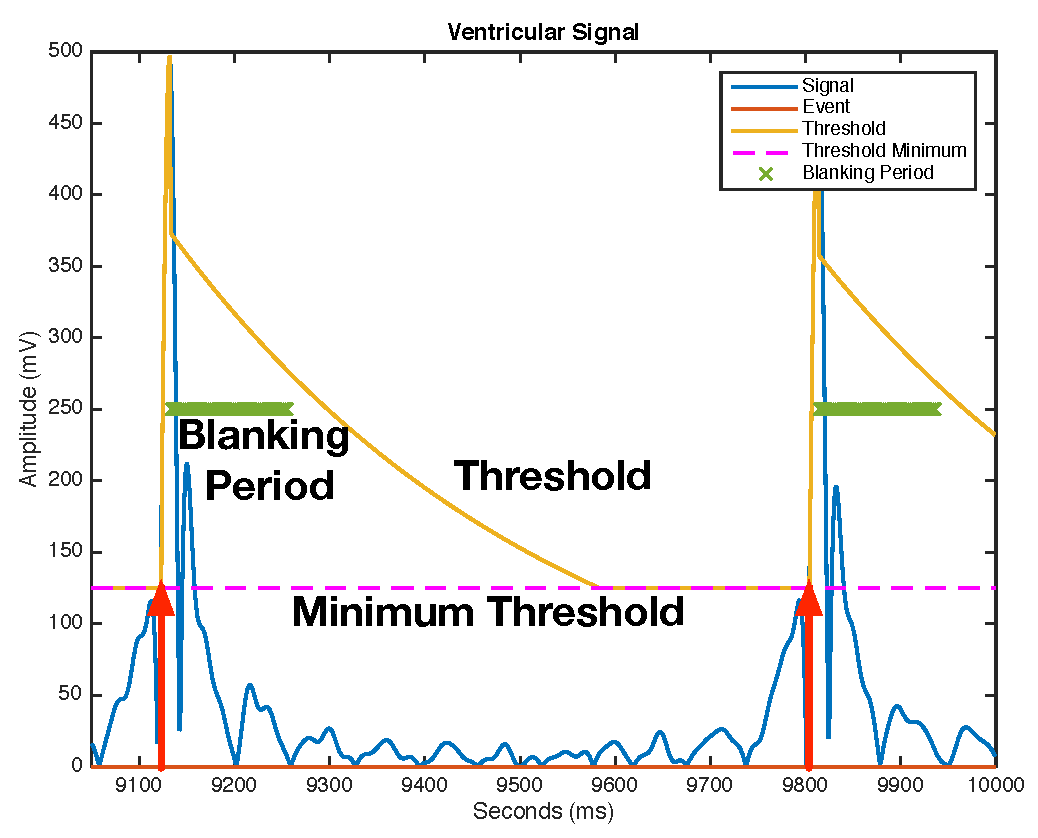
\includegraphics[scale=0.3]{figures/sensingExample}
	\vspace{-10pt}
	\caption{\small Example of dynamic threshold adjustment in ICD sensing algorithm. The shown signal is rectified.}
	\vspace{-10pt}
	\label{fig:sensingExample}
\end{figure}

\emph{Sensing} is the process by which cardiac signals $\egm$ measured through the leads of the \ac{ICD} are converted to timing events.
The \ac{ICD} declares events when the signal exceeds a dynamically-adjusted threshold $Th$.
%The threshold is dynamically adjusted in order to operate robustly in complex environments where cardiac events can vary greatly in signal amplitude and frequency, such as during \ac{VF}.

Fig. \ref{fig:sensingModel} shows the model $\Sys_{Sense}$ of the sensing algorithm, and Fig. \ref{fig:sensingExample} illustrates its operation. 
%In Fig. \ref{fig:overview} (ICD Sensing - $\Sys_{Sense}$), states not shown in a mode have a 0 derivative, e.g., $\dot{eF}=0$ in all modes. $y(t) = |\egm(t)|$.
The sensing takes place on the rectified \ac{EGM} signal $y = |\egm|$.
After an event is declared at the current threshold value ($y(t)\geq Th(t)$ in Fig. \ref{fig:sensingModel}), the algorithm tracks the signal in order to measure the next peak's amplitude \yhl{(Peak Tracking)}.
%During transition, the state to indicate peak discovery is reset ($f=0$). 
For a duration $MinTP$ (min tracking period) the latest peak is saved in $y_M$.
A variable $f$ indicates that a peak was found.
After a peak is found ($f==1$) and after the end of the tracking period, the algorithm enters a fixed \emph{Blanking Period} \yhl{(Blanking)}, during which additional events are ignored.
\yhl{On the transition to Blanking}, $Th$, $Th_0$ and the exponential factor of decay $eF$ is updated. 
At the end of the blanking period, the algorithm transitions to the Exponential Decay mode in which $Th$ decays exponentially from $Th_0$ to a minimum level \yhl{(Exponential Decay)}, and stays there for at least a sampling period of $MinDecP$.
Different manufacturers may use a step-wise decay instead of exponential, but the principle is the same.
%
Local peak detection is modeled via the $\dot{y} = 0 \wedge \ddot{y}<0$ transition.
While $y=|\egm|$ is non-differentiable at 0, the peak will occur away from 0, as shown in Fig. \ref{fig:sensingExample}.
The other states in Fig. \ref{fig:sensingModel} are $t, t_p$ (clocks).
$minTh$ and $TC$ are constant parameters.
\begin{thm}
	\label{thm:sensing}
	$\Sys_{Sense}$ is STORMED.	
\end{thm}
